\chapter{Scenario Series 6-6}

This document presents simulation results from the 6-6 scenario series, which tests impact of relaxing line-wise agent profitability constraint (both in bilevel anticipation, and in simulated agent behaviour). 
This simulates perfectly integrated (i.e., collaborative) agent fibre procurement behaviour, and makes it possible for the hardwood line to operate at a net loss if this is profitable for the network as a whole. 
This is a hypothetical scenario, as it makes optimistic assumptions regarding willingness of the hardwood line to operate at a net loss to benefit the rest of the network.
Some form of collaborative benefit-sharing agreement would have to been in place for this setup to be economically viable for the hardwood sub-agent, however no such agreements are in place in reality.

\section{Summary}
Table \ref{tab:scenario_list} below lists the scenarios in series 6-6. 

\begin{table}
  \centering
  \begin{tabular}{lll}
    \hline
    Scenario ID & Figure Reference & Description \\
    \hline
    6-6\_base & \ref{fig:s6-6_base} & Base scenario. \\
    \hline
  \end{tabular}
  \caption{Description of scenarios in series 6-6.}
  \label{tab:scenario_list}
\end{table}

\section{Results}

Figure \ref{fig:s6-6_base} presents
simulation results for fifteen scenarios. % Table \ref{tab:scenarios}
% summarizes scenario parameters used in the experiment for each
% scenario.
Disposition of figures is identical for all scenarios. The
first subfigure (a) for each scenario shows the initial
(ie. iteration-0) AAC solution. The second subfigure (b) for each
scenario shows first period of AAC solution for all 30 planning
iterations. The third subfigure (c) for each scenario shows the
implemented harvest level for all 30 planning iterations. Scenarios
3.1 and 3.2 also show profit in this subfigure on a secondary
axis. The fourth subfigure (d) for each scenario shows the difference
between initial and re-planned AAC. The fifth subfigure (e) for each
scenario shows the difference between re-planned AAC and harvest.  The
sixth subfigure (f) for each scenario shows the difference between
initial AAC and harvest. Softwood volume is shown with white bars,
hardwood volume with black bars, and total volume with small
circles. Profit (where applicable) is shown with the $\times$
symbol. 

\begin{figure}[h]
  \centering
  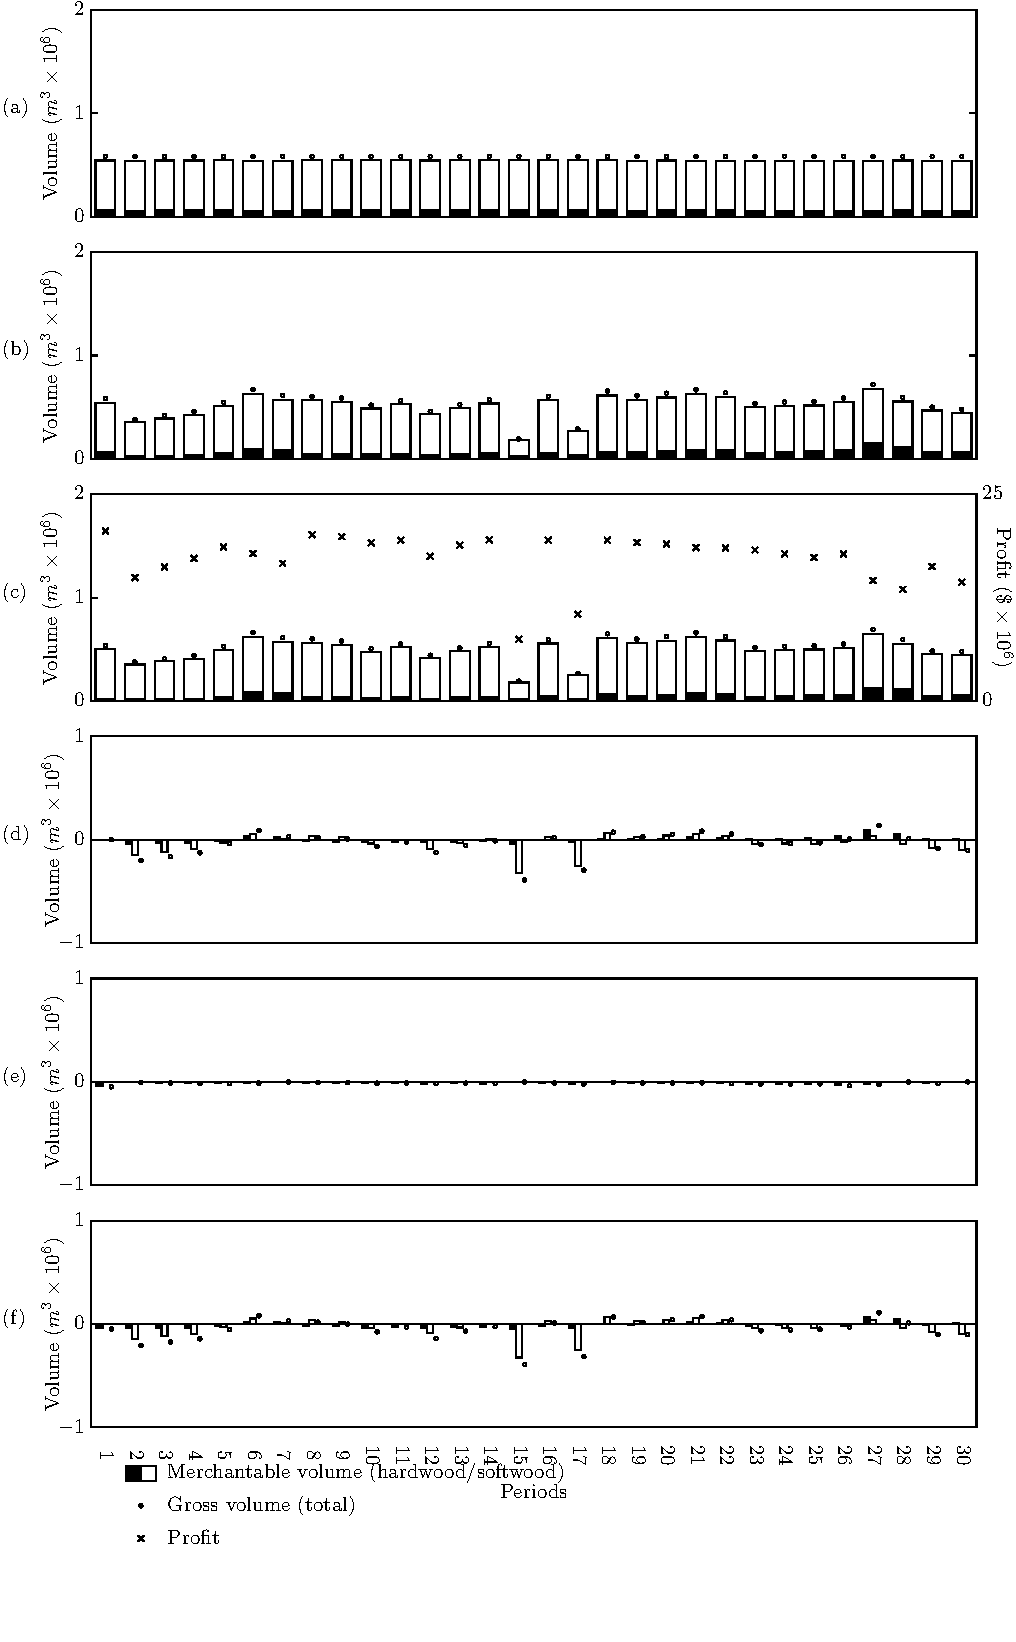
\includegraphics[width=10cm]{images/appendix/s6-6_base}
  \caption{Scenario 6-6\_base (base scenario).}
  \label{fig:s6-6_base}
\end{figure}

